\localauthor{Johann Schicho}

Im Folgenden ER-Diagramm sieht man die gesamte persistente Datenstruktur von LasEs. Die Kardinalität der \emph{Relationships} gibt die ganzzahligen Abhängigkeiten zwischen der einzelnen \emph{Entities} an. Die \emph{is-A} Spezialisierungen modellieren die unterschiedlichen Rollen/Typen einer Entität.

\begin{figure}[H]
	\centering
	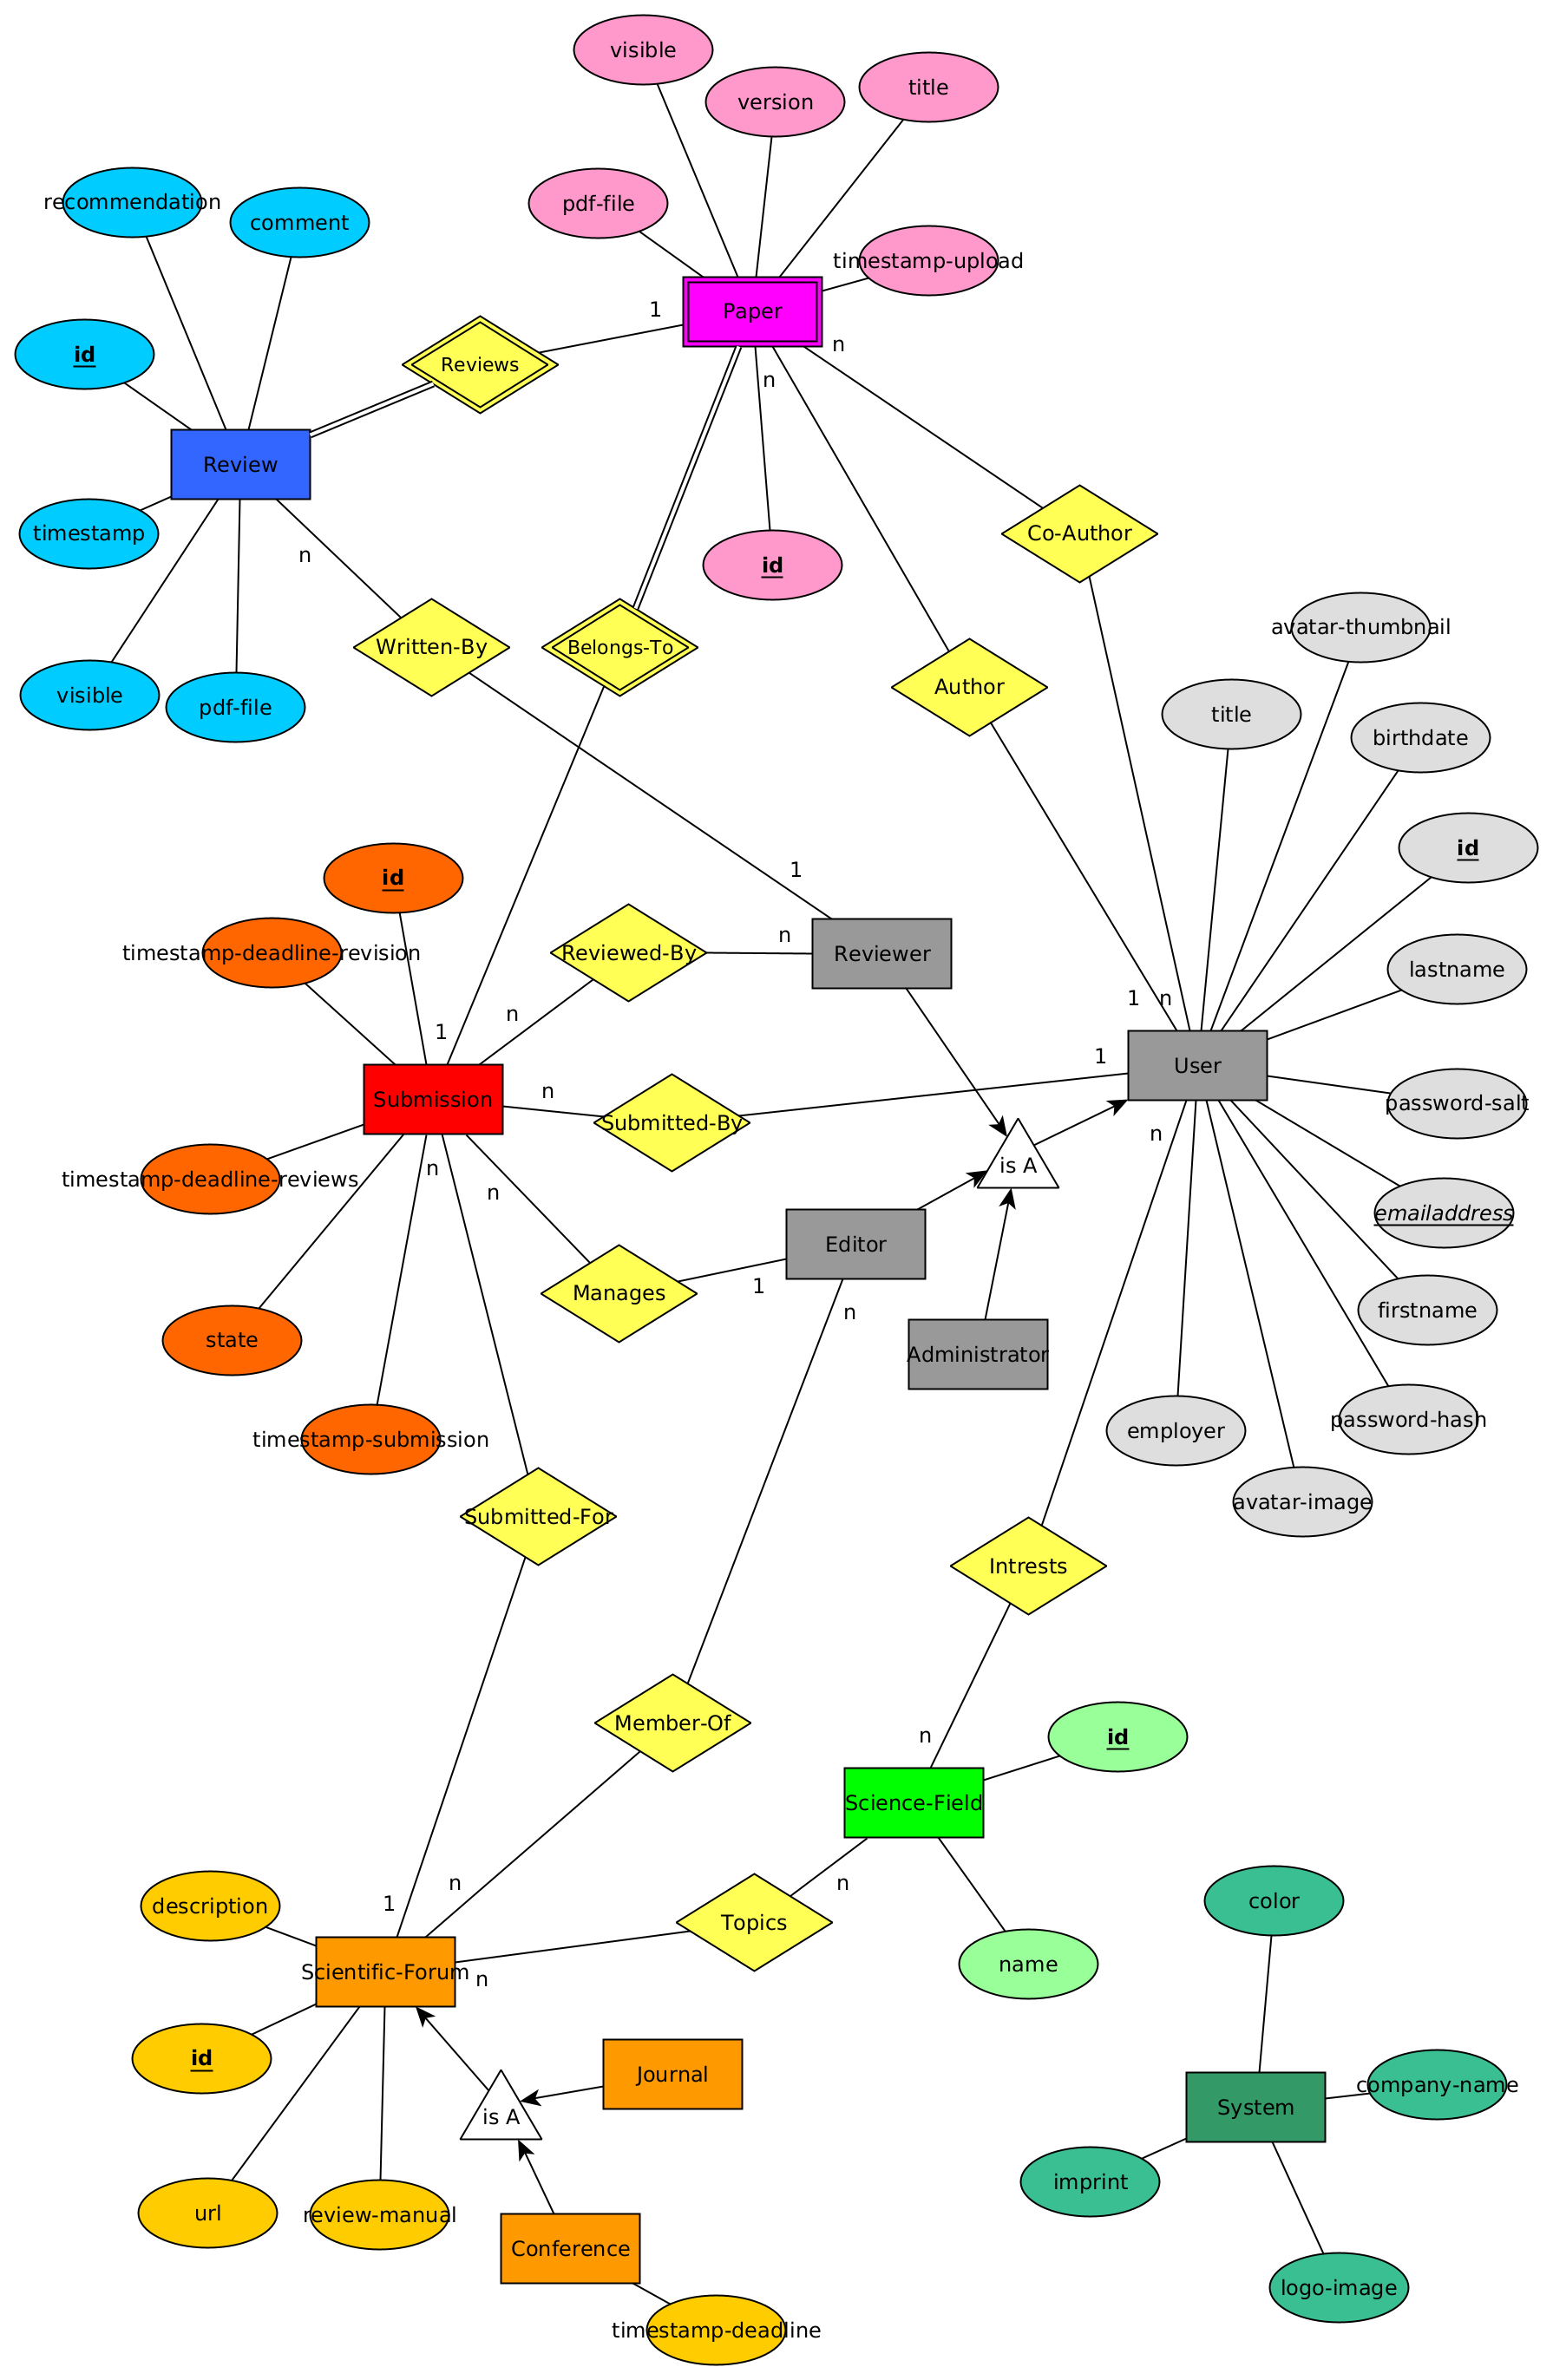
\includegraphics[width=\linewidth]{graphics/ER-Modell}
	\caption{Übersicht über die Zusammenhänge zwischen den Entitys}
	\label{er:diagramm}
\end{figure}